\section{Summary}
In this chapter we will use the textural developed in previous chapters 
to create a change detection algorithm (CDA). The CDA will be assessed
using the CARABAS-II image dataset, which is a set of images acquired by a Very High Frequency (VHF) Ultra Wideband (UWB) SAR system.
The CDA is based on the UNET convolutional neural network (CNN) architecture and will use the 
textural information as additional inputs for image classification.
It will be demonstrated that the 
use of textural information can improve the overall performance of the algorithm
in terms of probability of detection and false alarm rate. 

\section{Introduction}
As previously mentioned, SAR has several applications, such as, topology, oceonography, geology, environment monitoring, among others.
The SAR can operate in two modes: single-pass acquisition and multi-pass acquisition. In the first it is captured only one picture of the 
monitored area, while in the latter there can be multiple acquisitions of the same area. 
When dealing with multi-temporal acquisitions, we can either assess the information contained in the entire time frame or focus in detecting changes between the acquisitions. 
When the latter is the focus, change detection algorithms (CDA) are traditionally used to identify the relevant changes (ref carabas, ricardo).

Generally, CDA's priority is the percentage of true positives with a lower regard for percentage of false positives. 
Those can however be relevant in many applications such as detecting hidden objects over a large area, 
where a small number of false positives is vital in the quality of the final data for operation application - which is the main concern of this work. 
While trying to develop a CDA for this work, it was kept in mind that the CDA developed would have to provide a high percentage of true positives while trying to minimize
the amount of false positives.

The traditional method for creating CDAs was to base the decisor on standard statistical theory, e.g, traditional hypothesis testing criterion methods,
such as 
generalized likelihood ratio test ref{GLRT1,GLRT2,GLRT3}, 
maximum a posteriori criterion ref{Book May},
Bayesian theory approaches ref{Bayes1, Bayes2},
or likelihood ratio test ref{LRT1,LRT2,LRT3}. Even though these methods, most of the time, perform adequately in terms of probability of detection, but
most of them show poor performance in terms of false alarm rate (ref{Carabas, Ricardo,LucasRamos,Chris}). Those methods also have a few drawbacks, such as: depending on
additional preprocessing of the images throughout morphological operations (erosion and dilation filters have to normally be used) and depend on calibration of the algorithm
for the statistical analysis to work.

By trying to overcome the limitations of traditional statistical based CDAs, machine learning algorithms became popular in the last few years (ref Vinholi, Campos) since they
have the capability to perform better than statistical based CDAs and don't have the usual drawbacks that those methods present. There are two kinds of machine learning algorithms: supervised and unsupervised
algorithms. Supervised algorithms are the ones that have a  classification reference to help guide the learning step, while unsupervised algorithms are the ones that do not have this classification reference - 
on this work we focused only in supervised algorithms. As it was mentioned, it is important to know what is the parameter of interest to quantify the quality of the algorithm, e.g., we can assess performance
based on number of true positives, true negatives, false positives and false negatives (ref PefMe) - for this part of the work, the parameters of interest are number of true positives and number of false negatives.

Among supervised machine learning algorithms there are multiple algorithms that can be chosen to solve the problem, such as: Neural Networks, Naive Bayes, Linear Regression, Kernel Ridge Regression, Support Vector Machine, Decision Trees, Random Forest (ref PefMe).
For this work it was chosen to use a neural network based algorithm for the CDA. There are multiple types of neural networks, e.g., perceptron, Feed Forward Neural Network, Multilayer Perceptron, Recurrent Neural Network, Long Short-Term Memory Neural Network, convolutional
neural network, among others (ref PefMe). It was chosen to use a convolutional neural network, specifically a UNET convolutional neural network (Ref unet), for solving the target detection problem, since convolutional neural network have shown
excellent results for computer vision problems. In (ref Kevin) it was used a similar approach to detect change in SAR images, although in (ref Kevin) the SAR images were acquired in a much higher frequency. 
  
The UNET CNN will not only have the SAR acquisitions as input for the target detection, but will also have textural information that will be extracted according to the methods explained in 
chapter 3. 
In (ref rodrigo) it was already shown that additional textural information can provide valuable information to improve classification results. It is important to mention that since CNN use convolutions, which are linear filters, to achieve better classification results,
it would be redundant to use linear textural information as inputs to the UNET CNN.  When comparing the proposed technique with other algorithms on the same dataset, we show that the results show similar detection performance but presenting a significant false alarm rate improvement.

\section{Relevant Textures for the Change Detection Algorithm}
As it was done in (ref rodrigo) we will use the method of Sum and Difference Histograms to compute the textures (ref sarker), since they have been demonstrated to compute 
useful textures to be used as additional information for machine learning algorithms and it is a texture computation method that can run in linear time. We will again give a brief overview of the method.

For a given SAR image, we consider the random variable $u_{[x, y]}$ to be the absolute value of the backscatter value received by the antenna. The first step of the algorithm is to 
quantize the random variable $u$ to have $N_g$ discrete integer possible values (on this work $N_g$ was chosen to be 20). The second step is to obtain an estimate of the joint probability density function of the random v $[u_{[x,y]}, u_{[x+\delta x, y+\delta y]}]$ (where $\delta = (\delta x, \delta y)$ is the displacement vector 
chosen to compute the texture direction and distance),
which is a $N_g \times N_g$ matrix. According to (ref Unser), it is possible to create an estimate of this Joint PDF in linear time by creating a random gaussian vector that has uncorrelated, therefore independent, random variables, and then computing the textures 
directly from the two linear independent variables. The new vector is $[s_{[x,y]}, d_{[x, y]}]$ and is obtained as follows:

\begin{equation}
    \begin{array}{ccc}
         s_{[x,y]} &=& u_{[x,y]} + u_{[x+\delta x, y+\delta y]} \\
         d_{[x,y]} &=& u_{[x,y]} - u_{[x+\delta x, y+\delta y]}
    \end{array}.
\end{equation} 

Since $s_{[x,y]}$ and $d_{[x,y]}$ are independent, it is possible to decompose the original Joint PDF as the product of two PDF as follows:
\begin{equation}
    \begin{array}{rrr}
       P(u_{[x,y]}=u_1, u_{[x+\delta x, y+\delta y]}=u_2) = \\ P(s_{[x,y]}=u_1+u_2, d_{[x,y]}=u_1-u_2) = \\
    P(s_{[x,y]}=u_1+u_2) \cdot P(d_{[x,y]} = u_1-u_2) 
    \end{array}
\end{equation}

By doing this it is now possible to compute the textures directly from the random variables $P_s$ and $P_d$. Notice that by doing this, the time 
complexity of the texture calculation was reduced from $O(N_g^2)$ to $O(2*N_g)$.

After obtaining the probability density functions $P(s_{[x,y]})$ and $P(d_{[x,y]})$, a set of textural information can be extracted as follows (for better readability, we define $P_s(i) = P(s[x,y] = i)$ and $P_d(j) = P(d[x,y] = j))$:
\begin{enumerate}
    \item Mean($\mu$): describes the mean value of the co-occurrences and is given by
    \begin{equation}
        \textrm{MEAN} = \frac{1}{2}\sum_{i=1}^{N_g}i\cdot P_s(i)
    \end{equation}
    
    \item Cluster prominence: describes the fourth moment of the random variables and is given by
    \begin{equation}
        \textrm{CLP} = \sum_{i=1}^{N_g}(i-2\mu)^4\cdot P_s(i)
    \end{equation}
    
    \item Cluster shade: describes the third moment of the random variables and is given by
    \begin{equation}
        \textrm{CLS} = \sum_{i=1}^{N_g}(i-2\mu)^3\cdot P_s(i)
    \end{equation}
    
    \item Contrast: measure the difference of intensities of co-occurrences in the image and is given by
    \begin{equation}
        \textrm{CON} = \sum_{j=\frac{-N_g}{2}}^{\frac{N_g}{2}}(j)^\cdot P_d(j)
    \end{equation}
    
    \item Correlation: describes the linear correlation of intensities of co-occurrences in the image and is given by
    \begin{equation}
        \textrm{COR} = \frac{1}{2}\sum_{i=1}^{N_g}(i-2\mu)^2\cdot P_s(i)-\frac{1}{2}\sum_{j=\frac{-N_g}{2}}^{\frac{N_g}{2}}(j)^\cdot P_d(j)
    \end{equation}
    
    \item Energy: describes the energy of the received signal and is given by
    \begin{equation}
        \textrm{ENE} = \sum_{i=1}^{N_g}P_s(i)^2\cdot \sum_{j=\frac{-N_g}{2}}^{\frac{N_g}{2}} P_d(j)^2
    \end{equation}
    
    \item Entropy: describes the uncertainty of the co-occurrence matrix and is given by
    \begin{equation}
        \textrm{ENT} = -\sum_{i=1}^{N_g}P_s(i)\log(P_s(i)) - \sum_{j=\frac{-N_g}{2}}^{\frac{N_g}{2}} P_d(j)\log(P_d(j))
    \end{equation}
    
    \item Homogeneity: describes the degree of similarity between images and is given by
    \begin{equation}
        \textrm{HOM} = - \sum_{j=\frac{-N_g}{2}}^{\frac{N_g}{2}} \frac{P_d(j)}{1+j^2}
    \end{equation}
    
    \item Variance: describes the degree of dispersion of intensities between two images and is given by
    \begin{equation}
        \textrm{VAR} = \frac{1}{2} \sum_{i=1}^{N_g}(i-2\mu)^2 P_s(i) + 
         \frac{1}{2}\sum_{j=\frac{-N_g}{2}}^{\frac{N_g}{2}} j^2 P_d(j)
    \end{equation}
\end{enumerate}

There are multiple textures that can be chosen as additional inputs for the UNET CNN. One have to keep in mind, that, for every texture that it is used as additional information, 
the time computation for the training and validation of the UNET will be also increased, so it is vital to keep in mind the trade-off between computation time and improvement of classification results.

For this work it was chosen to use the Entropy and Variance images textures as additional information. The original picture and the texture pictures can be seen in Fig. \ref{fig:exemplo_carabas}, Fig. \ref{fig:entropy_example} and Fig. \ref{fig:variance_example}.

\begin{figure}[h]
    \centering
    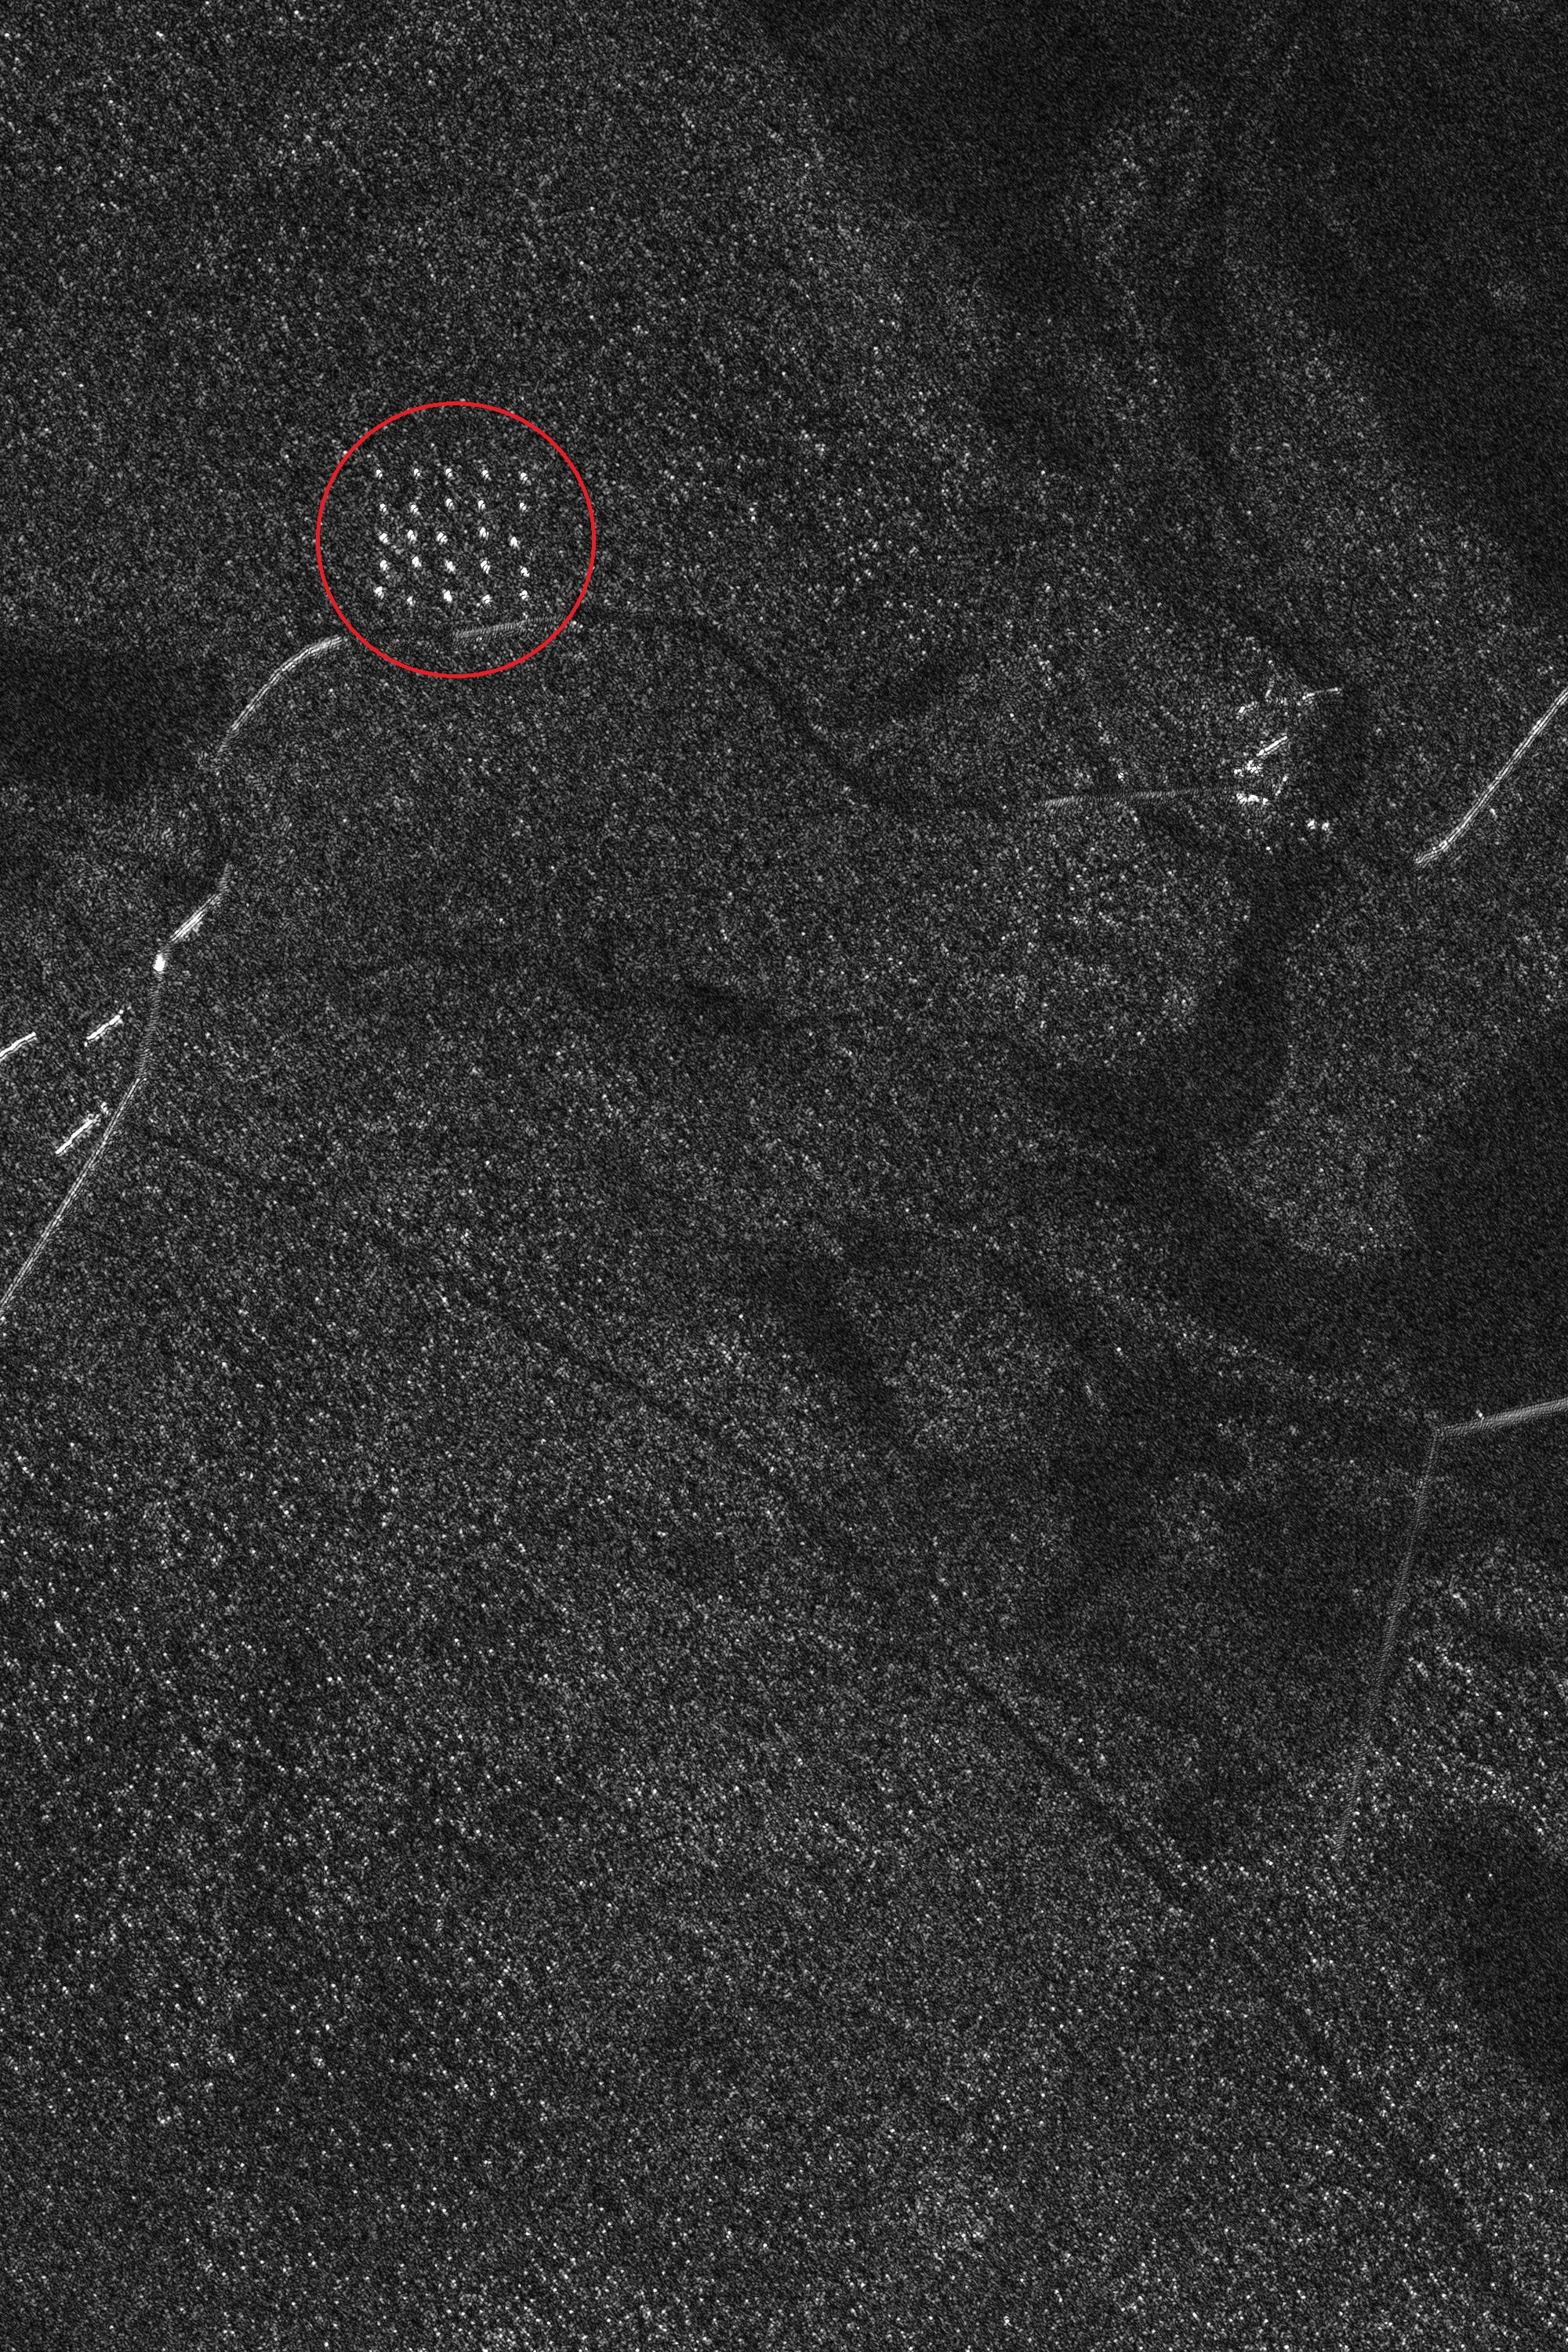
\includegraphics[width=0.45\linewidth]{Chapter7/exemplo_carabas.jpg}
    \caption{ Example of a SAR image acquired by the CARABAS-II system.
    The red circle shows the position of the cars hidden under a canopy of trees.}
    \label{fig:exemplo_carabas}
\end{figure}

\begin{figure}[h]
    \centering
    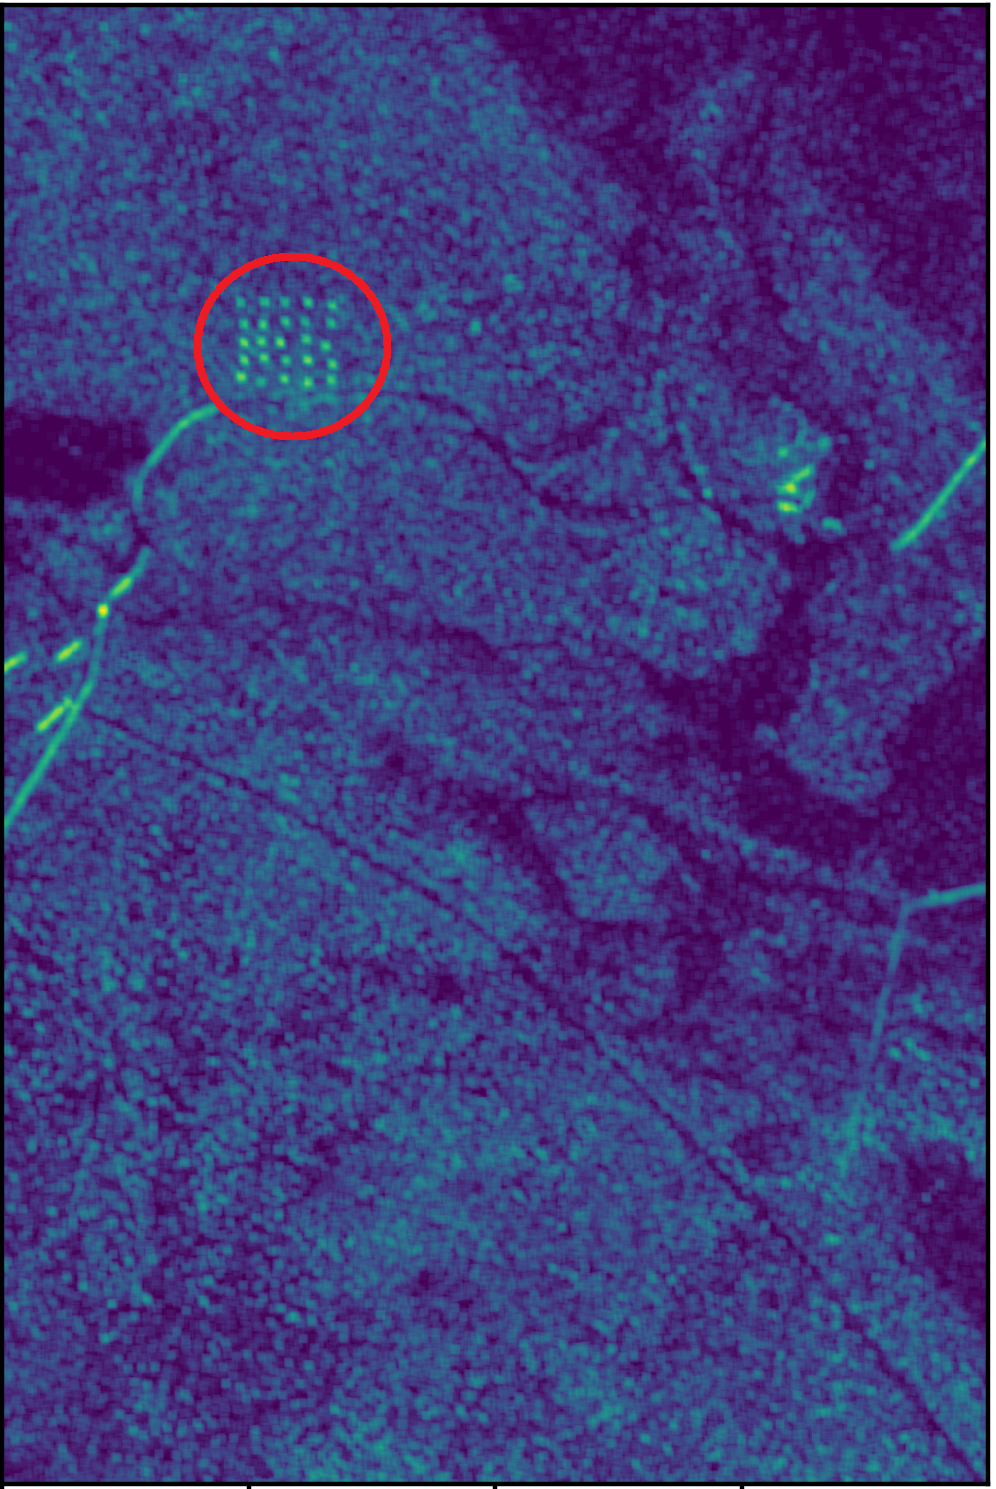
\includegraphics[width=0.45\linewidth]{Chapter7/entropy_examplepng.png}
    \caption{Entropy image. The red circle shows the position of the vehicles.}
    \label{fig:entropy_example}
\end{figure}

\begin{figure}[h]
    \centering
    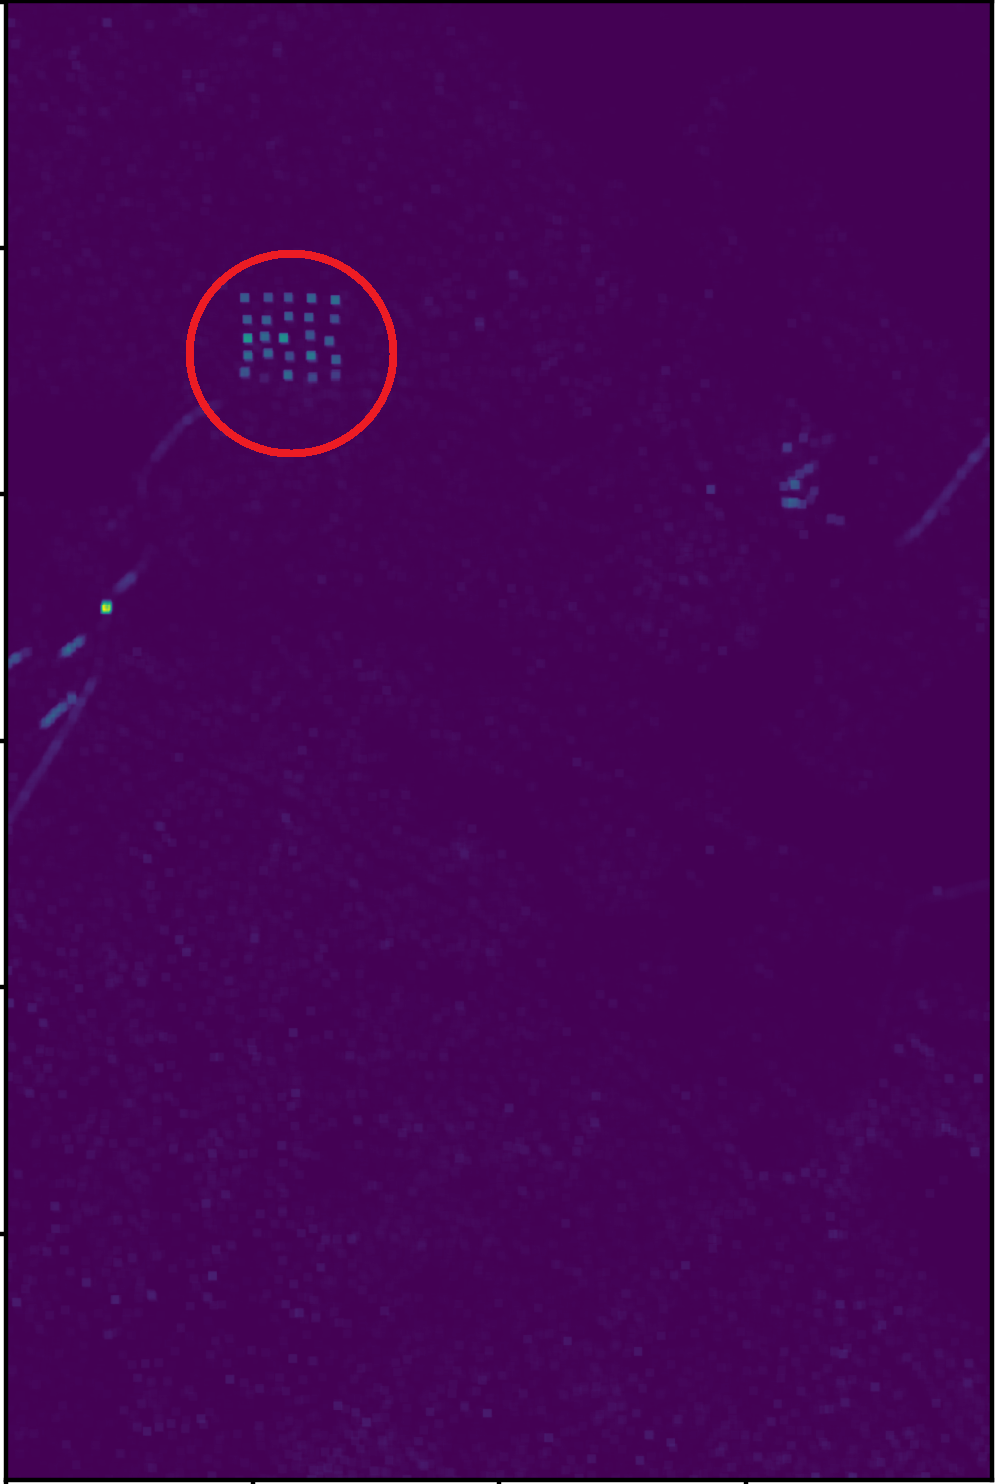
\includegraphics[width=0.45\linewidth]{Chapter7/variance_exemplo.png}
    \caption{Variance image. The red circle shows the position of the vehicles}
    \label{fig:variance_example}
\end{figure}

\section{UNET Based Algorithm for Target Change Detection}
\section{Results}
